\documentclass[tikz,border=8pt]{standalone}
\usepackage{tikz}
\usepackage{xcolor}
\usepackage{amsmath}
\usepackage{amsfonts, amssymb}
\pagecolor{black}
\color{white}

\begin{document}
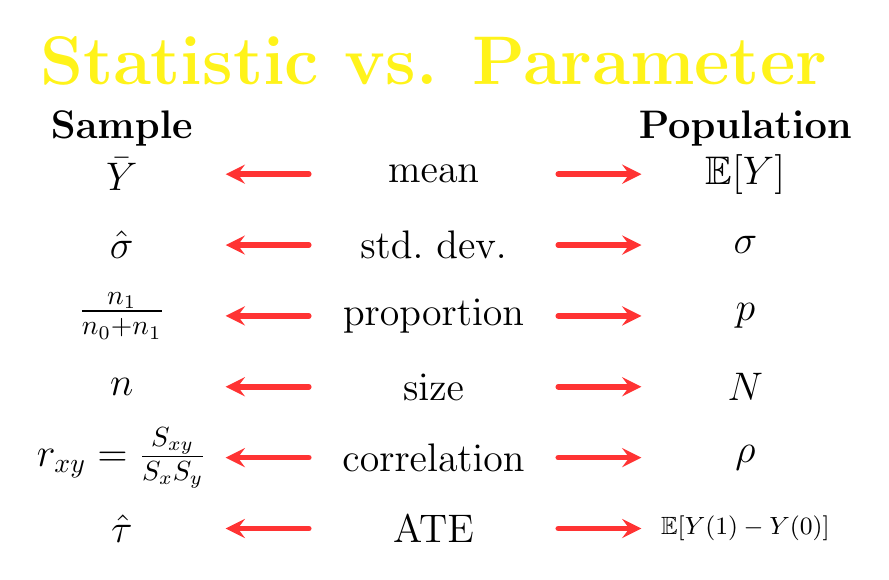
\begin{tikzpicture}[>=stealth, line cap=round, xscale=.33, yscale=.45]

% --- layout helpers ---
\def\L{-12.0}   % left column x
\def\C{0}      % center column x
\def\R{12.0}    % right column x

% --- title ---
\node[text=yellow!90!white, align=center, font=\bfseries\fontsize{34}{38}\selectfont]
  at (\C,9.2) {Statistic vs. Parameter};

% --- column headers ---
\node[font=\bfseries\Large] at (\L,7.3) {Sample};
\node[font=\bfseries\Large] at (\R,7.3) {Population};
% \draw[blue!60, line width=1.2pt] (-15,6.9) -- (-9.5,6.9);
% \draw[blue!60, line width=1.2pt] (9.5,6.9) -- (15,6.9);

% --- a small macro for each row: center label + red arrows to L/R, white symbols ---
\newcommand{\rowitem}[4]{%
  % y, center label, left symbol, right symbol, (optional) tweak for center font size
  \node[font=\Large] at (\C,#1) {#2};
  \node[font=\Large] at (\L,#1) {#3};
  \node[font=\Large] at (\R,#1) {#4};
  \draw[red!80,->,line width=2pt] (\C-4.8,#1) -- (\L+4,#1);
  \draw[red!80,->,line width=2pt] (\C+4.8,#1) -- (\R-4,#1);
}

% --- rows (top to bottom) ---
% Mean
\rowitem{6.0}{mean}{$\bar{Y}$}{$\mathbb E[Y]$}

% Standard deviation
\rowitem{4.0}{std.\ dev.}{$\hat \sigma$}{$\sigma$}

% Proportion
\rowitem{2.0}{proportion}{$\frac{n_1}{n_0 + n_1}$}{$p$}

% Size
\rowitem{0.0}{size}{$n$}{$N$}

% Correlation (useful in SBS)
\rowitem{-2.0}{correlation}{$r_{xy} = \frac{S_{xy}}{S_x S_y}$}{$\rho$}

% ATE (Average Treatment Effect; SBS-relevant)
\rowitem{-4.0}{ATE}{$\hat{\tau}$}{\small $\mathbb E[Y(1) - Y(0)]$}

\end{tikzpicture}
\end{document}

